\documentclass{scribe}

%====================================================================
%====================================================================
% IMPORTANT: PLEASE UPDATE THE LECTURE INFORMATION BELOW:
\setcounter{lecture}{24} % Lecture number here, from The Big Table on Canvas
\renewcommand{\lectureTitle}{Digital Signatures, Modeling Digital Signatures, RSA Signatures}
\renewcommand{\lecturer}{Mahdi Cheraghchi}
\renewcommand{\scribe}{Yi-Wen Tseng}
\renewcommand{\lectureDate}{April 5, 2023} % Date of the lecture
%====================================================================
%====================================================================

\begin{document}

\maketitle

%=============================================================================
%=============================================================================

\section{Continue on Better RSA Encryption Approach}
Apply $RSA_{N,e}$ on a random $x \leftarrow \mathbf{Z}_N^*$. Then, we know $x$ is hard to recover from $y=RSA_{N,e}(x)$.
\\
We first use a hash function on $x$ and encrypt message $m$:
\[c = (y=RSA_{N,e}(x) = x^e \bmod N, H(x) \oplus m)\]  
\\
$Dec(sk=(N,d), c=(y,p))$: Compute $x=RSA_{N,d}(y) = y ^d \bmod N$ and output $H(x) \oplus p$. This mechanism meets the correctness requirement.
\vspace{8mm}
\\
We also need to check security requirement of RSA.
\\\\
\textbf{CPA Security}: Hash function (really random like)
\\
A good hash function "practically behaves" like a uniform random function (a.k.a random oracle) e.g. SHA-3 is quite "random-like"
\\
\begin{figure}[H]
    \centering
    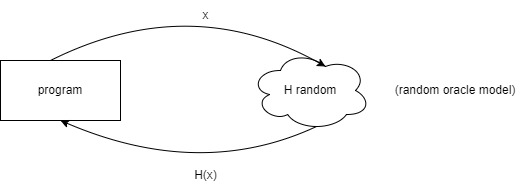
\includegraphics[scale=0.5]{rsa_encryption.jpg}
    \caption{RSA Encryption}
\end{figure}
\noindent Because $x$ is unknown, $H(x)$ would be close to completely unknown. Thus, it is stronger than collision resistance. In the other words, because x is not fully known to the adversary, $H(x)$ is completely random. On the other hand, if the adversary knows $x$, then they also completely know $H(x)$.
\\\\
\textbf{Theorem}: If RSA assumption holds (factoring is hard) and $H$ is a "random oracle," then RSA encryption is CPA secure. 
\vspace{10mm}
%=============================================================================
%=============================================================================
\section{Digital Signature}
In Diffie-Hellmen, we solve the encryption problem, but there is still integrity problem. The good news is RSA can be used in both encryption and integrity, which is referred to as \textbf{digital signature}.
\\\\
Digital signature can help us authenticating the identiy of the sender under public key setting.
\\
For example,
\begin{itemize}
    \item A person's ID should be verifiable as authentication by everyone (attested by the governments)
    \item Crypto wallet
    \item A financial digital contract
    \item signed email
\end{itemize}
\vspace{10mm}
%=============================================================================
%=============================================================================
\section{Modeling Digital Signature}
The digital signature is similar to MAC.
\\\\
Signature scheme: $\pi = (Gen, Sign, Ver)$ with interface:
\begin{itemize}
    \item $Gen(1^n)$: Output a (public) verification key $v_k$ and a (secret) signing key $s_k$
    \item $Sign(s_k,m)$: Given signing key $s_k$ and message $m$, output signature $\sigma$
    \item $Ver(v_k,m,\sigma)$: Given verification key message $m$,  purported signature $\sigma$, accept or reject
\end{itemize}
\vspace{5mm}
We need to check the correctness and the security of RSA digital signature:
\begin{itemize}
    \item Correctness\\
            $\forall (v_k,s_k) \leftarrow Gen(1^n)$, $\forall m, Ver(v_k,m,Sign(s_k,m))=\text{ always accept}$
    \item Security\\
            We need to show that the digital signature is unforgeable under Chosen Message Attack (CMA game).\\\\
            \textbf{Definition}: A sign scheme $\pi = (Gen,Sign,Ver)$ is UFCMA if $\forall \text{ p.p.t forger} F$:
            \[Adv_{\pi}^{CMA} = \Pr_{(v_k,s_k) \leftarrow Gen(1^n)}(F^{Sign_{s_k}(.)}(1^n,v_k) \text{ forges}) = negl(n) \]
            where forging means outputing $(m^*,\sigma^*)$ such that:
            \begin{enumerate}
                \item $Ver(v_k,m^*,\sigma^*) = $ accept
                \item $m^*$ wasn't a query to the $Sign_{s_k}(.)$ oracle
            \end{enumerate}
            For "strong" unforgeability, we relax the second criteria to be $(m^*,\sigma^*)$ wasn't a query-answer pair.  
\end{itemize}

\vspace{10mm}
%=============================================================================
%=============================================================================
\section{RSA Signature}
RSA Signature is literally the reverse of RSA encryption.
\subsection{Textbook Version of RSA Signature}
\begin{itemize}
    \item $Gen(1^n)$: run $(N,e,d) \leftarrow GenRSA(1^n)$, output $v_k = (N,e)$ and $s_k = (N,d)$
    \item $Sign(s_k=(N,d), m \in \mathbf{Z}_N^*)$: output $\sigma = RSA_(N,d)(m) = m^d \bmod N = RSA_{(N,e)}^{-1}(m)$
    \item $Ver(v_k=(N,e), m \in \mathbf{Z}_N^*, \sigma \in \mathbf{Z}_N^*)$: accept if and only if $m=RSA_{N,e}(\sigma) = \sigma^e \bmod N$, else reject
\end{itemize}
\begin{figure}[H]
    \centering
    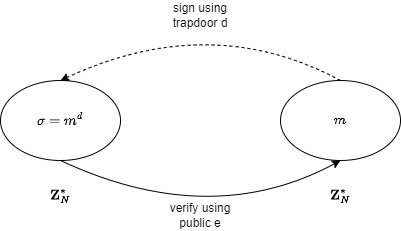
\includegraphics[scale=0.5]{rsa_signature.jpg}
    \caption{RSA Digital Signature}
\end{figure}
The mechanism meets the correctness requirement, but it is not unforgeable. 
\\
In fact, it is forgeable with zero queries. The forger first choose any $\sigma^* \in \mathbf{Z}_N^*$ and compute $m^* = RSA_{(N,e)}(\sigma^*) = (\sigma^*)^e \bmod N$. Then, it outputs $(m^*, \sigma^*)$ to the verifier.
\\\\
A more threatening forgery can work as follows:
The forger qeuries two times to get $(m, \sigma)$ and $(m^{'},\sigma^{'})$.
Then, the forger computes a new valid message-signature pair by doing:
\[ m^* = m \cdot m^{'} \]
\[\sigma^{*} = \sigma \cdot \sigma^{'} \in \mathbf{Z}_N^*\]
We can check the signature:
\[(\sigma^{*})^e = \sigma^e \cdot \sigma^{'e} = m \cdot m^{'} = m^{*} (\bmod N)\]
\vspace{5mm}
\subsection{A Better Version of RSA Signature}
\begin{figure}[H]
    \centering
    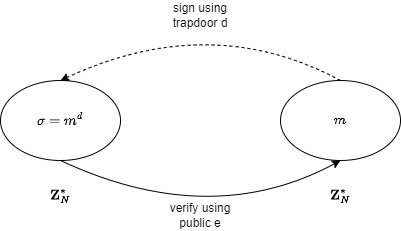
\includegraphics[scale=0.5]{rsa_signature.jpg}
    \caption{RSA Digital Signature}
\end{figure}
Similar to RSA Encryption, we use a collision resistant hash function $H$ to introduce randomness.
\begin{itemize}
    \item $Gen(1^n)$: run $(N,e,d) \leftarrow GenRSA(1^n)$, output $v_k = (N,e)$ and $s_k = (N,d)$
    \item $Sign(s_k=(N,d), m \in \mathbf{Z}_N^*)$: output $\sigma = RSA_(N,d)(H(m)) = H(m)^d \bmod N = RSA_{(N,e)}^{-1}(H(m))$
    \item $Ver(v_k=(N,e), m \in \mathbf{Z}_N^*, \sigma \in \mathbf{Z}_N^*)$: accept if and only if $H(m) = \sigma^e \bmod N  = RSA_{N,e}(\sigma)$
\end{itemize}
\textbf{Theorem}: Under RSA assumption, this "hash and sign" signature is UFCMA if $H$ is modeled as a "random oracle" eahc query $(m_i, \sigma_i)$ is distributed like random. In other words, $H(m_i) = \sigma_i^e \bmod N$ for random $\sigma_i$ tells forger nothing.
\\
\textbf{Caveat}: For real functions, $H:{0,1}^* \rightarrow \mathbf{Z}_N^*$ should "cover" all of $\mathbf{Z}_N^*$. For instance, SHA-3 gets 256-bit outputs, but RSA needs 4096-bit module. To make hash longer, we use "repeated hashing."
\vspace{10mm}
%=============================================================================
%=============================================================================

%\lipsum

%=============================================================================
%=============================================================================

\bibliographystyle{alpha}
% Uncomment below if you have any references:
%\bibliography{\jobname}

%=============================================================================
%=============================================================================

\end{document}
